% -*- mode:flyspell; mode:latex -*-
\documentclass[12pt]{article}
\addtolength{\oddsidemargin} {-0.885in}
\addtolength{\textwidth}{1.75in}
\addtolength{\evensidemargin}{-0.8in}


\usepackage[latin1]{inputenc}
\usepackage[T1]{fontenc}
\usepackage[english]{babel}
\usepackage{graphicx}
\usepackage{float}
%% \usepackage{siunitx}

%% \usepackage{gensymb}


\usepackage{tikz}
\usepackage{[caption}
\usetikzlibrary{arrows}
\usetikzlibrary{decorations.markings}
\usetikzlibrary{decorations.pathmorphing}
% \usepackage[absolute,overlay]{textpos}
% \usepackage{onimage}

\usepackage{tabularx}
\usepackage{times}
\usepackage{graphics}

% \usepackage{subfigure}
% \usepackage{scalefnt}
%
% \renewcommand\thesubfigure{\arabic{subfigure}}

\usepackage{amsmath}
\usepackage{hyperref}
\usepackage{hhline}
\usepackage{subfig}
\usepackage{color}
\usepackage[all]{hypcap}

\usepackage[normalem]{ulem}  % for striking out
% \usepackage{fancyhdr}
% \pagestyle{fancy}
% \fancyhead[C]{}
% \fancyhead[L] {\it{Mu2e-doc-29670-v1.0} }
%%%%%%%%%%%%%%%%%%%%%%%%%%%%%%%%%%%%%%%%%%%%%%%%%%%%%%%%%%%%%%%%%%%%%%%%%%%%%%
% use natbib - biblatex not available on Mu2e interactive nodes
%%%%%%%%%%%%%%%%%%%%%%%%%%%%%%%%%%%%%%%%%%%%%%%%%%%%%%%%%%%%%%%%%%%%%%%%%%%%%%
\usepackage[square,sort,comma,numbers]{natbib}

% location of the .bib files: env var BIBINPUTS (~/library/bibliography)

% \usepackage[backend=biber, style=numeric-comp, sorting=ynt] {biblatex}
% \addbibresource{clfv.bib}

% \addbibresource{stntuple.bib}
% \addbibresource{mu2e_web.bib}
% \addbibresource{radiative_pion_capture.bib}

\graphicspath{{figures/}}
%%%%%%%%%%%%%%%%%%%%%%%%%%%%%%%%%%%%%%%%%%%%%%%%%%%%%%%%%%%%%%%%%%%%%%%%%%%%%%
% for portability, make sure all commands are included locally,
%%%%%%%%%%%%%%%%%%%%%%%%%%%%%%%%%%%%%%%%%%%%%%%%%%%%%%%%%%%%%%%%%%%%%%%%%%%%%%
\definecolor{ForestGreen}{RGB}{30,139,30}
%\include{commands}
\newcommand {\blue}      {\color{blue}}
\newcommand {\green}     {\color{ForestGreen}}
\newcommand {\red}       {\color{red}}
\newcommand {\purple}    {\color{purple}}
\newcommand {\violet}    {\color{violet}}

\newcommand {\kmax}      {\mbox{$k_{\rm max}$}}
\newcommand {\mumemconv}[1][A] {\mbox{$\mu^- \textrm{#1} \rightarrow e^- \textrm{#1}$}}
% Define a relay to have 2 default arguments instead of limit of 1
\newcommand {\mumepconv}[1][A] {%
  \def\ArgI{{#1}}%store the first argument
  \mumepconvRelay
}
\newcommand \mumepconvRelay[1][A]  {\mbox{$\mu^- \textrm{\ArgI} \rightarrow e^+ \textrm{#1}$}}
\newcommand {\MuToEm}     {\mbox{$\mu^- \ra e^-$}}
\newcommand {\MuToEp}     {\mbox{$\mu^- \ra e^+$}}
\newcommand {\MuPToEp}    {\mbox{$\mu^+ \ra e^+$}}
\newcommand {\ra}        {\rightarrow}
\newcommand {\Rmue}       {\mbox{$R_{\mu e}$}}
\newcommand {\tandip}    {\mbox{$\tan \lambda$}}

\newcommand {\Pb}[1]     {\mbox{$\rm ^{#1}Pb$}}                 % isotopes of lead
\newcommand {\Au}[1]     {\mbox{$\rm ^{#1}Au$}}                 % isotopes of gold
\newcommand {\Ir}[1]     {\mbox{$\rm ^{#1}Ir$}}                 % isotopes of iridium
%%%%%%%%%%%%%%%%%%%%%%%%%%%%%%%%%%%%%%%%%%%%%%%%%%%%%%%%%%%%%%%%%%%%%%%%%%%%%%
% editing commands
%%%%%%%%%%%%%%%%%%%%%%%%%%%%%%%%%%%%%%%%%%%%%%%%%%%%%%%%%%%%%%%%%%%%%%%%%%%%%%
\newcommand {\del}[1]    {{\blue \sout{#1}}}
\newcommand {\dlt}[1]    {{\violet \sout{#1}}} %alternate delete color
\newcommand {\add}[1]    {{\red #1}}
\newcommand {\alt}[1]    {{\green #1}} %alternate comment color
%%%%%%%%%%%%%%%%%%%%%%%%%%%%%%%%%%%%%%%%%%%%%%%%%%%%%%%%%%%%%%%%%%%%%%%%%%%%%%
\begin{document}

\begin{titlepage}
  \begin{flushright}
    \bf {MU2E/PHYSICS/37812} \\
    version 1.01
    \today
 \end{flushright}

  \vspace{1cm}

  \begin{center}
    {\Large \bf On the feasibility of using $\pi^+ \to e^+ \nu$ decays \\
      for momentum scale calibration of the Mu2e tracker

      \vspace{0.3in}
      10. subtitle
    }

    \vspace{1cm}
    P.Murat(FNAL), S.Tripathy(UC Davis)

    % \footnote{\texttt{Fermilab; e-mail: murat@fnal.gov}}
    \vspace{0.3cm}

    \vspace{0.8cm}
  \end{center}

  \begin{abstract}

    \vspace{0.2in}
    The dominant background is expected to come from muon decays in flight.
    To the extent to which one can rely on the Geant4 simulation of the low momentum
    pion production , one caWe show that irreducible background in 
  \end{abstract}

\end{titlepage}
% \frontmatter
% \chapter*{Abstract}
%
% \addcontentsline{toc}{chapter}{Abstract}
%
% \mainmatter
%
{\tableofcontents}

%%%%%%%%%%%%%%%%%%%%%%%%%%%%%%%%%%%%%%%%%%%%%%%%%%%%%%%%%%%%%%%%%%%%%%%%%%%%%%%
%\chapter{Calibration}
%%%%%%%%%%%%%%%%%%%%%%%%%%%%%%%%%%%%%%%%%%%%%%%%%%%%%%%%%%%%%%%%%%%%%%%%%%%%%%%
% \input{input_data}

%%%%%%%%%%%%%%%%%%%%%%%%%%%%%%%%%%%%%%%%%%%%%%%%%%%%%%%%%%%%%%%%%%%%%%%%%%%%%%%

\newpage
\section {Revision History}

\begin{itemize}
\item
\item
  v1.01: inital version
\end{itemize}

\section {Introduction}

Feasibility of using $\pi^+ \to e^+\nu$ for calibrating the momentum scale of the Mu2e tracker
has been investigated by several groups -see \cite{UB_NOTES, PURDUE_NOTES} and references therein.

Presently, the ultimate conclusion remains somewhat uncertain.
Several issues , however, are understood:
\begin{itemize}
\item 
  study of the $\pi^+ \to e^+\nu$ channel requires performing the measurement at early times.
  That requires sigreducing the proton beam proton beam intensity to be significantly reduced. 
  That allows not to worry too much about the pileup
\item
  to reduce the background from muon decays in flight, this calibration requires
  special instrumentation, a beam degrader, to be installed in the DS.
\end{itemize}

%%%%%%%%%%%%%%%%%%%%%%%%%%%%%%%%%%%%%%%%%%%%%%%%%%%%%%%%%%%%%%%%%%%%%%%%%%%%%%
\section{Simulation of the $\pi+ \to e^+ \nu $ signal }

{\red Briefly Describe the multistage simulation - standard Mu2e scheme
  \begin{itemize}
  \item
    first: simulation of pion beam
  \item
    then - simulation of the $\pi^+ \to e^+ \nu$ decays in the detector
  \end{itemize}
}
%%%%%%%%%%%%%%%%%%%%%%%%%%%%%%%%%%%%%%%%%%%%%%%%%%%%%%%%%%%%%%%%%%%%%%%%%%%%%% 
\subsection {Pion lifetime: validation}

Weighting events with the pion lifetime - validation plot here

\begin{figure}[H]
  \begin{tikzpicture}
    \node[anchor=south west,inner sep=0] at (0,0.) {
      % \node[shift={(0 cm,0.cm)},inner sep=0,rotate={90}] at (0,0) {}
      \makebox[\textwidth][c] {
        \includegraphics[width=1.0\textwidth]{pdf/missing_plot}
      }
    };
    \node [text width=8cm, scale=1.0] at (14.5,0.5) {$\mu_B$, expected background mean};
    \node [text width=8cm, scale=1.0, rotate={90}] at (1.5,7.5) { $S_{D}$, ``discovery'' signal strength  };
  \end{tikzpicture}
  \caption{
    \label{fig:pion_lifetime}
  }
\end{figure}

To increase statistics, the pion beam simulation had the charged pion decays turned off.
The survival probability of stopped $\pi^+$'s was stored and used in the analysis
as the event weight.

%%%%%%%%%%%%%%%%%%%%%%%%%%%%%%%%%%%%%%%%%%%%%%%%%%%%%%%%%%%%%%%%%%%%%%%%%%%%%% 
\subsection{Comparison to the BU analysis}

{\red 
\begin{itemize}
\item 
  Compare the signal yield/POT  - should be stable enough.
\item
  BU number : (after all cuts - mu2e-5391 , what are they?): $2.3 x 10^{-12}$ / POT
\end{itemize}
}


%%%%%%%%%%%%%%%%%%%%%%%%%%%%%%%%%%%%%%%%%%%%%%%%%%%%%%%%%%%%%%%%%%%%%%%%%%%%%% 
\section {Muon decays in flight and the degrader thickness}


%%%%%%%%%%%%%%%%%%%%%%%%%%%%%%%%%%%%%%%%%%%%%%%%%%%%%%%%%%%%%%%%%%%%%%%%%%%%%%
\subsection {Constraining the muon proper decays time - validation}



%%% Local Variables:
%%% mode: latex
%%% TeX-master: "mu2e-xxxxx"
%%% End:

%%%%%%%%%%%%%%%%%%%%%%%%%%%%%%%%%%%%%%%%%%%%%%%%%%%%%%%%%%%%%%%%%%%%%%%%%%%%%% 
\section {Other background sources}
\begin{itemize}
\item
  $\pi^+ \to \mu^+ \nu \to e^+ \nu \nu $ in the ST
  energy conservation : extends up to the $\pi^+ \to e^+ \nu$ peak, but not higher
  
  large BR, suppressed by the muon lifetime, phase space
  
\item
  $\pi^+ \to \mu^+ \nu \to e^+ \nu \nu $ in the degrader. The same argumens
\item
  decays of stopped $\mu^+$ : nominally end at 52.8
\end{itemize}

%%% Local Variables:
%%% mode: latex
%%% TeX-master: "mu2e-xxxxx"
%%% End:

%%%%%%%%%%%%%%%%%%%%%%%%%%%%%%%%%%%%%%%%%%%%%%%%%%%%%%%%%%%%%%%%%%%%%%%%%%%%%%
\newpage
\section {Reconstruction }

Distributions of the reconstructed track momentum and T0 for all reconstructed positive
tracks from $\pi^+ \to e^+ \nu $ decays in the ST are shown in Figure~\ref{fig:all_tracks_p_t0}.
The distributions corresponding to different degrader thicknesses are overlaid.
One can see that the probability per POT to have a reconstructed positron track reaches its maximum
for degrader thicknesses of about 2-3 mm Ti, and it starts falling down as the degrader thickness
increases.

Compared to ``no degrader'', a 2-3mm thick Ti degrader increases the acceptance by a factor
close to x3.

\begin{figure}[H]
  % \centering
  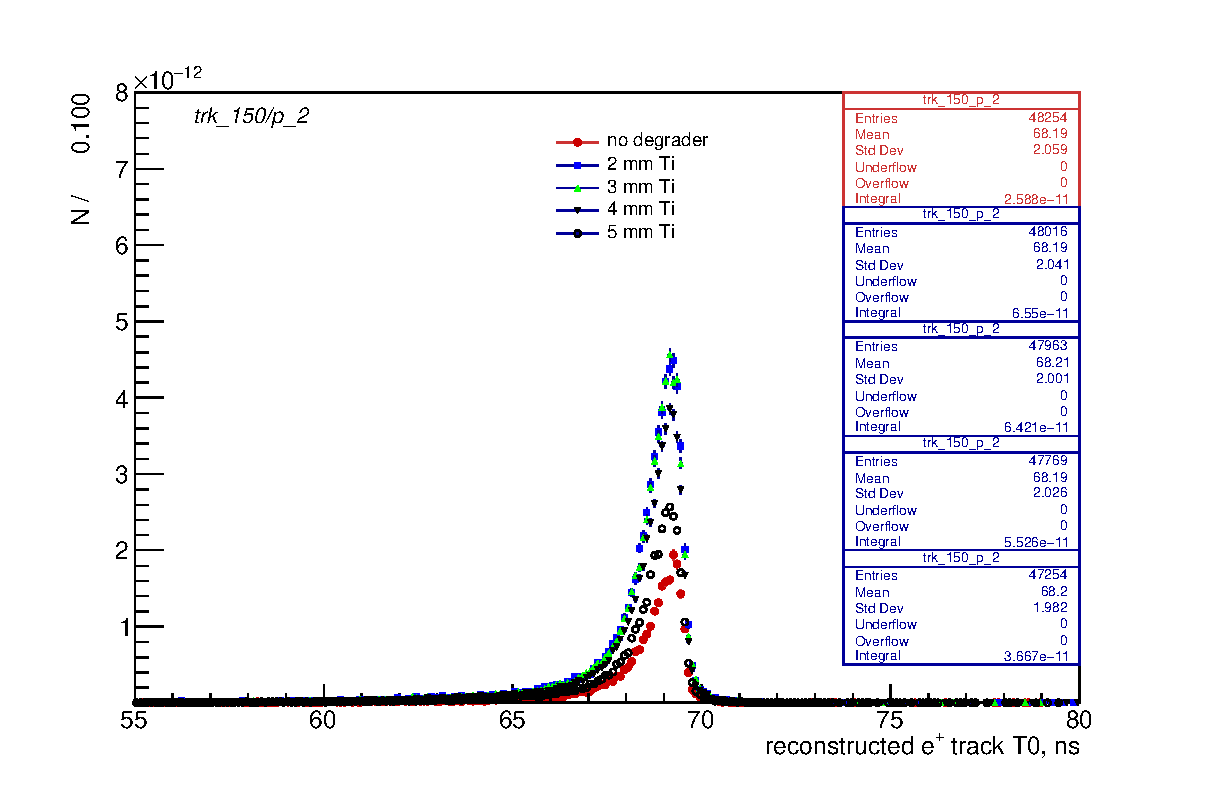
\includegraphics[width = 0.55\linewidth]{pdf/figure_00001}
  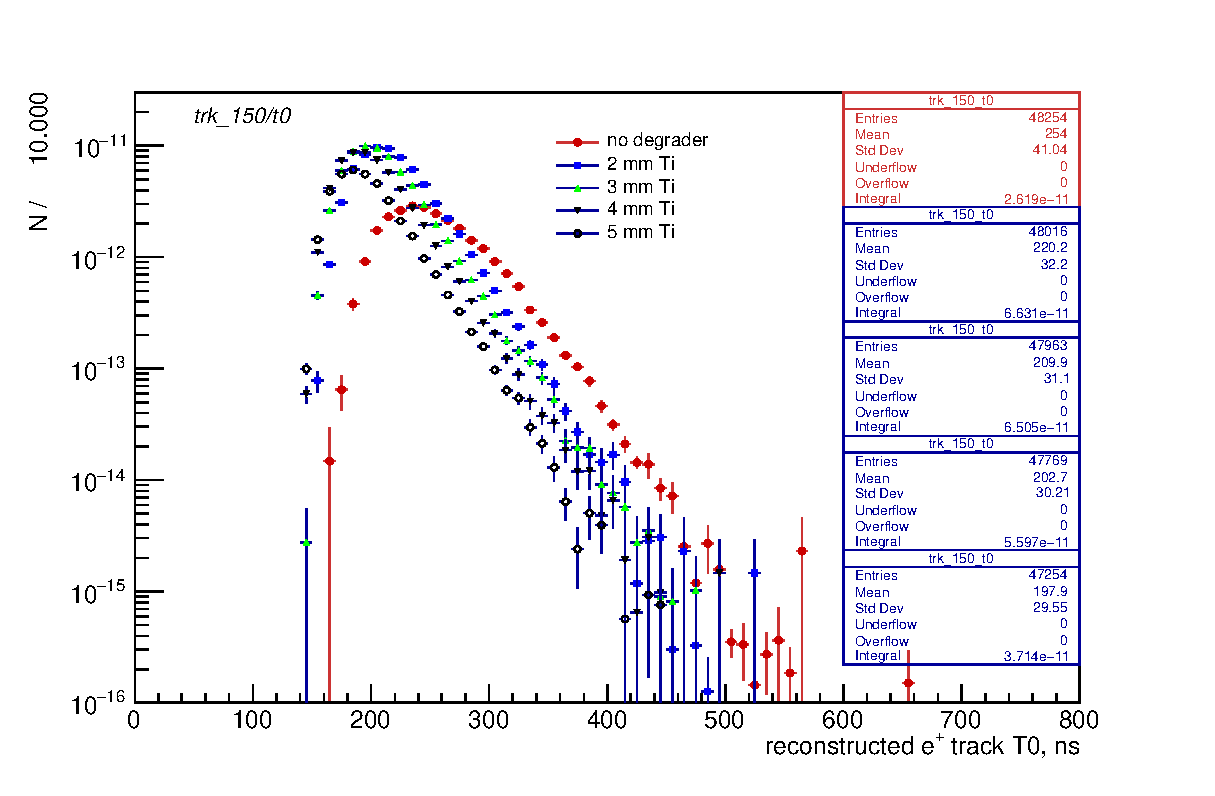
\includegraphics[width = 0.55\linewidth]{pdf/figure_00002}
  \caption{
    \label{fig:all_tracks_p_t0}
    Distributions of the reconstructed ST $\pi^+ \to e^+ \nu$ track momentum and time
    for different degrader thicknesses
  }
\end{figure}

%%%%%%%%%%%%%%%%%%%%%%%%%%%%%%%%%%%%%%%%%%%%%%%%%%%%%%%%%%%%%%%%%%%%%%%%%%%%%%
\subsection{Track selection cuts}

Based on the distributions in the track ID variables presented in Figure~\ref{fig:tid_variables_2mm},
we adopt the track ID cuts shown in the Table~\ref{table:track_id_cuts}

The cut values are very close to an old set of cuts known as "Set C" \cite{MU2E:3996:CutsetC}
and used by previous analyses, so a similar selection efficiency should be expected.

Cuts on $\tan \lambda$ and the track $d0$ provide significant rejection of the DIF
and $\pi \to e \nu$ decays in the degrader.

\begin{figure}[H]
  % \centering
  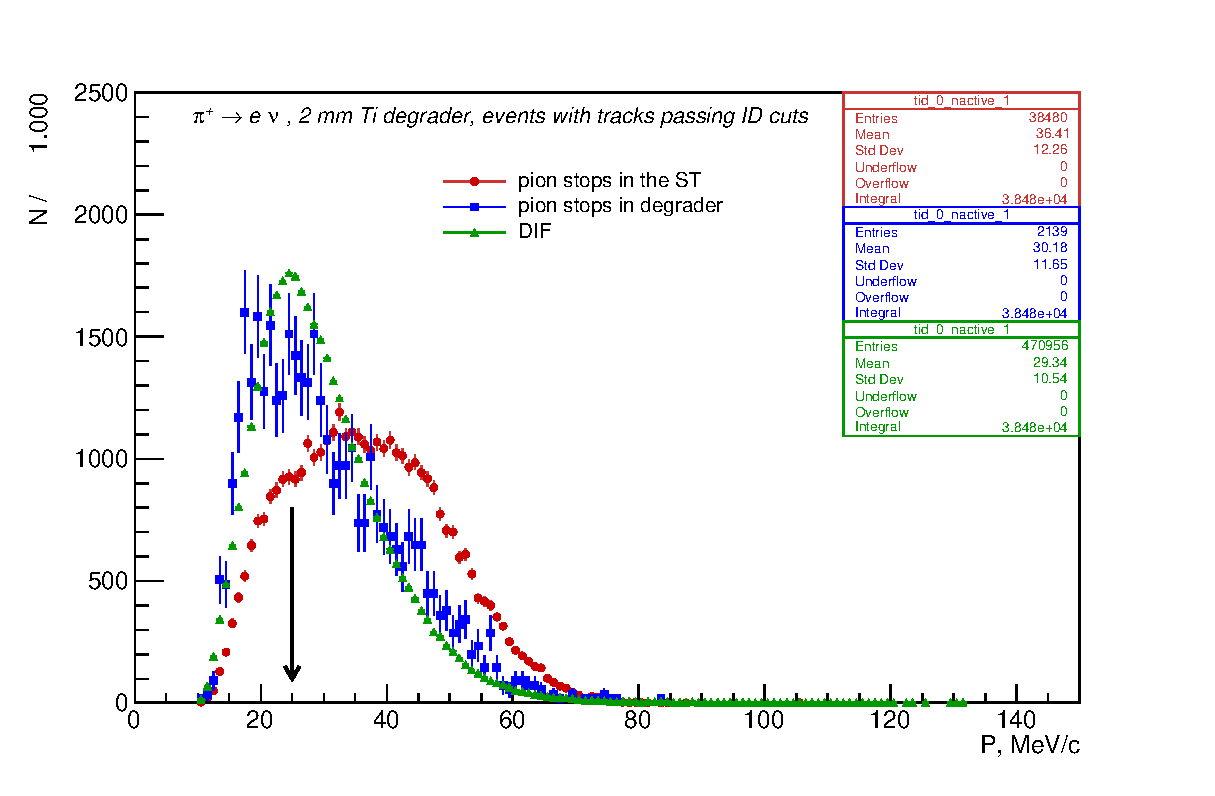
\includegraphics[width=0.55\linewidth]{pdf/figure_00274}  % tid_0/nactive_1
  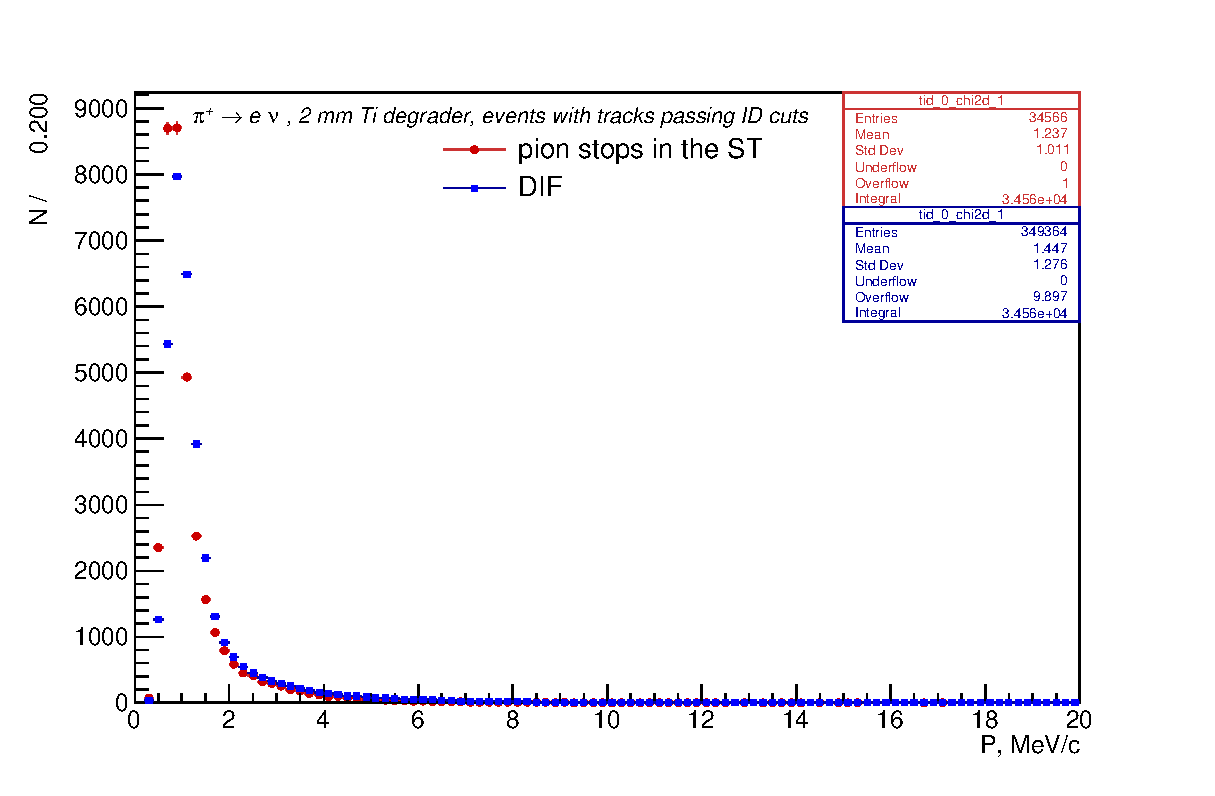
\includegraphics[width=0.55\linewidth]{pdf/figure_00275}  % tid_0/chi2d_1
  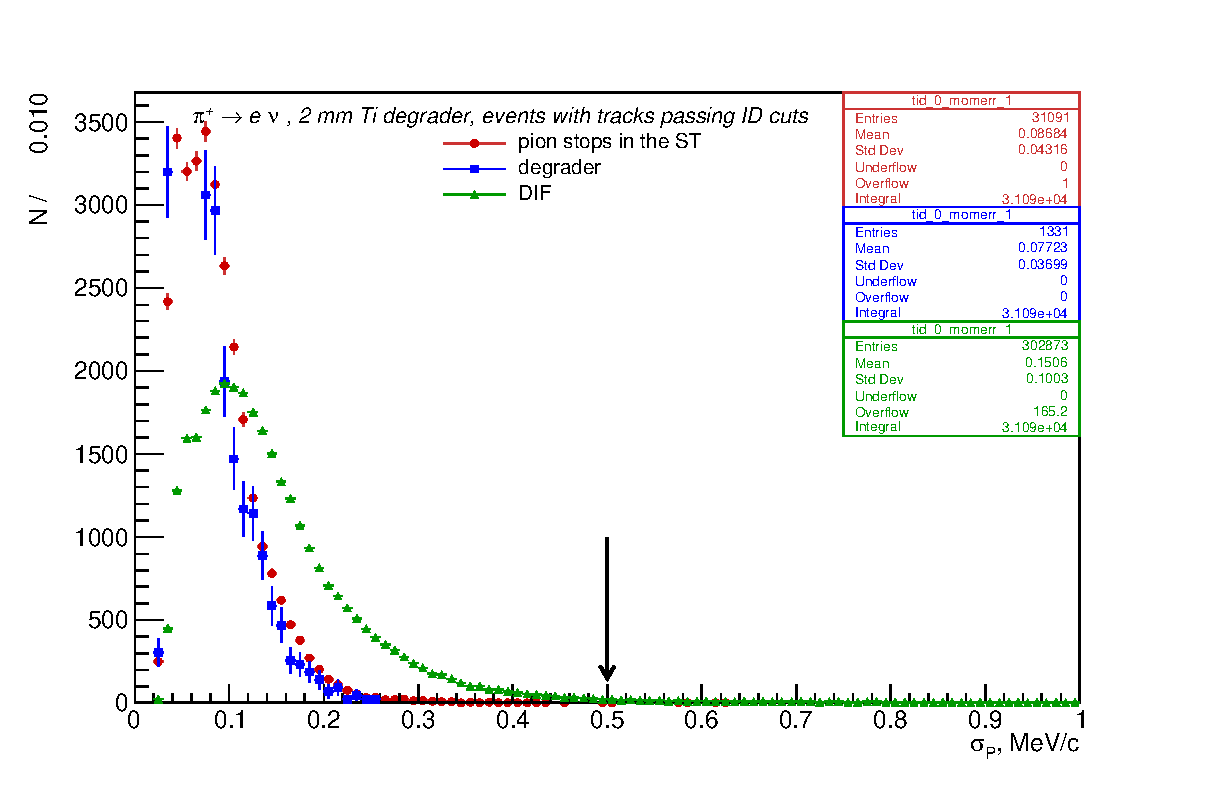
\includegraphics[width=0.55\linewidth]{pdf/figure_00276}  % tid_0/momerr_1
  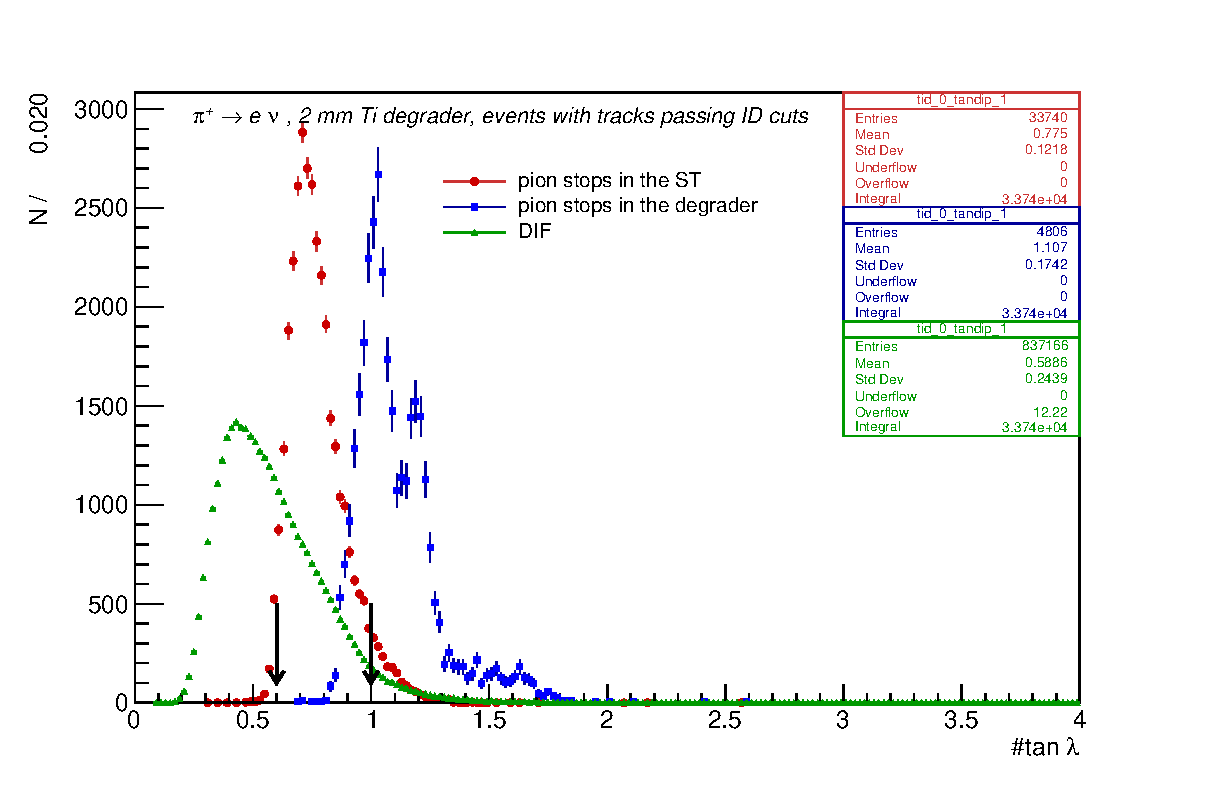
\includegraphics[width=0.55\linewidth]{pdf/figure_00273}  % tid_0/tandip_1
  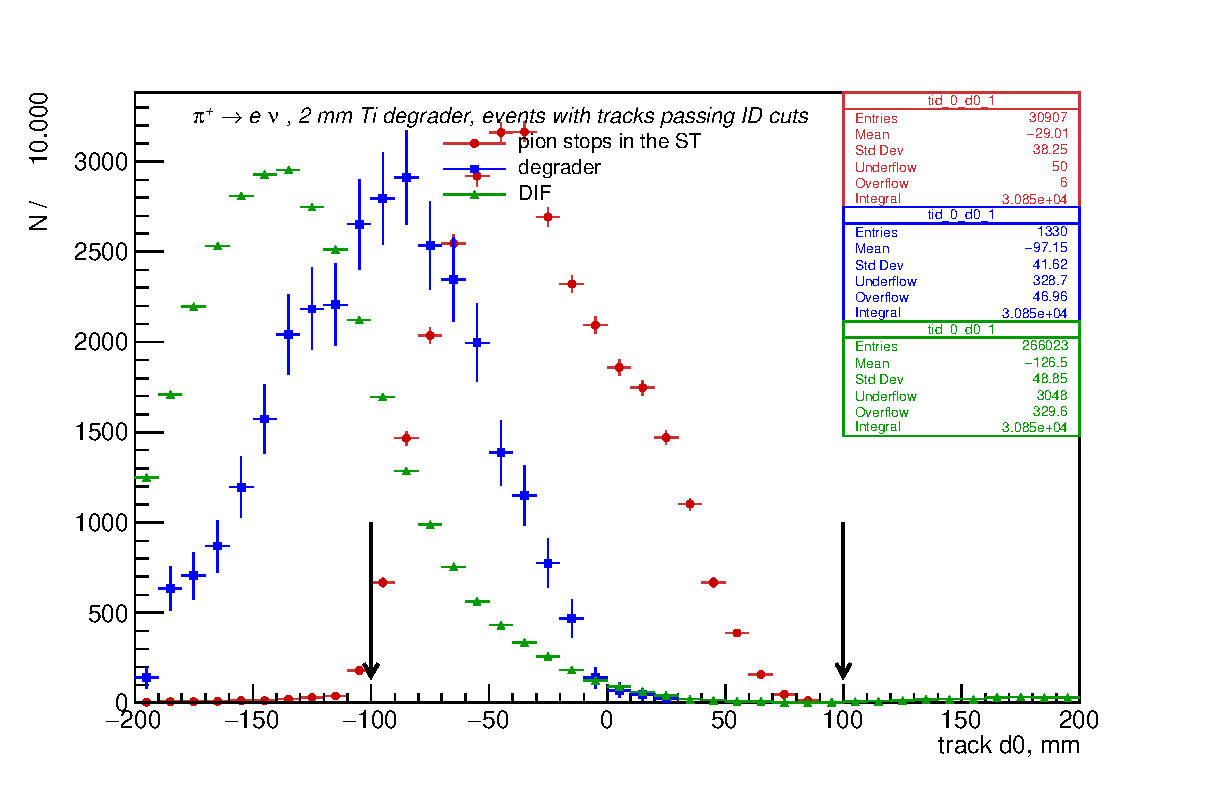
\includegraphics[width=0.55\linewidth]{pdf/figure_00277}  % tid_0/d0_1
  \caption{
    \label{fig:tid_variables_2mm}
    Distributions of the track ID variables for the 2mm Ti degrader
  }
\end{figure}

\begin{table}[H]
  \centering
  \begin{tabularx} {0.5\textwidth}{|X|c|}  %
    \hline
    variable                &   cut                        \\
    \hline                         
    N hits used by the fit  &   $N_{active}>= 25$            \\
    \hline                         
    chi2/DOF                &   $\chi2/DOF < 3$            \\
    \hline                         
    track dip angle         &   $0.6 < \tan \lambda < 1.0$ \\
    \hline                         
    track momentum error    &   $\sigma_P < 0.25$ MeV/c     \\
    \hline                         
    track $d_0$             &   $-100 < d_0 < 100$ mm     \\
    \hline
  \end{tabularx}
  \caption{
    \label{table:track_id_cuts}
    Track ID cuts
  }
\end{table}

It is worth noticing that the cut on the track dip angle significantly reduces
the contribution of positrons coming from $\pi^+ \to e^+ \nu$ decays in the degrader.

%%%%%%%%%%%%%%%%%%%%%%%%%%%%%%%%%%%%%%%%%%%%%%%%%%%%%%%%%%%%%%%%%%%%%%%%%%%%%%
\subsection{Signal reconstruction efficiency}

%% to see the number of entries and the weight, plot murat_pipenu_ana:trk_150/p_2

As shown in Table~\ref{table:reconstruction_eff}, the probability to reconstruct
a positron track from \piplusenu\ decay
is slightly below 50\% and it only marginally depends on teh thickness of the degrader.

\begin{table}[H]
\begin{tabularx}{1.0\textwidth} {|X|c|c|c|c|c|}  %
% \begin{tabular}{1.0\textwidth} {|l|l|}  %
  \hline
 degrader thickness &   Dataset  & probability for       &N $\pi^+$&N simulated  &N(reco tracks)     \\
 (mm)               &            & $\pi^+$ to stop in ST & stops   & \piplusenu\ &    ST             \\
  \hline                                                                                  
  no degrader       &   bpip0b0  &   4.23e-07            &  312616 &  100000     &   48254           \\
  \hline                                                                                  
     2              &   bpip2b0  &   1.11e-06            &   84785 &  100000     &   48016          \\
  \hline                                                                                  
     3              &   bpip3b0  &   1.09e-06            &   50340 &  100000     &  47963           \\
  \hline                                                                                  
     4              &   bpip4b0  &   9.44e-07            &   31681 &  100000     &  47769           \\
  \hline                                                                                  
     5              &   bpip5b0  &   6.35e-07            &   17225 &  100000     &  47254            \\
  \hline
\end{tabularx}
  \caption{
    \label{table:reconstruction_eff}
    Number of the events with reconstructed tracks for different pion datasets
  }
\end{table}

%%%%%%%%%%%%%%%%%%%%%%%%%%%%%%%%%%%%%%%%%%%%%%%%%%%%%%%%%%%%%%%%%%%%%%%%%%%%%%
\newpage
\subsection{Decays of pions stopped in the degrader}

Momentum distributions for reconstructed positron tracks from $\pi^+ \to e^+ \nu$ decays
in the ST and degrader are shown in Figure~\ref{fig:stt_vs_deg_momentum_good_tracks}.
The tracks are required to pass the selection cuts listed in Table~\ref{table:track_id_cuts}.
The selection efficiency is slightly higher than 60\%.

%%%%%%%%%%%%%%%%%%%%%%%%%%%%%%%%%%%%%%%%%%%%%%%%%%%%%%%%%%%%%%%%%%%%%%%%%%%%%%%
% before the selections cuts - all tracks - don't need
%%%%%%%%%%%%%%%%%%%%%%%%%%%%%%%%%%%%%%%%%%%%%%%%%%%%%%%%%%%%%%%%%%%%%%%%%%%%%%%
% \begin{figure}[H]
%   % \centering
%   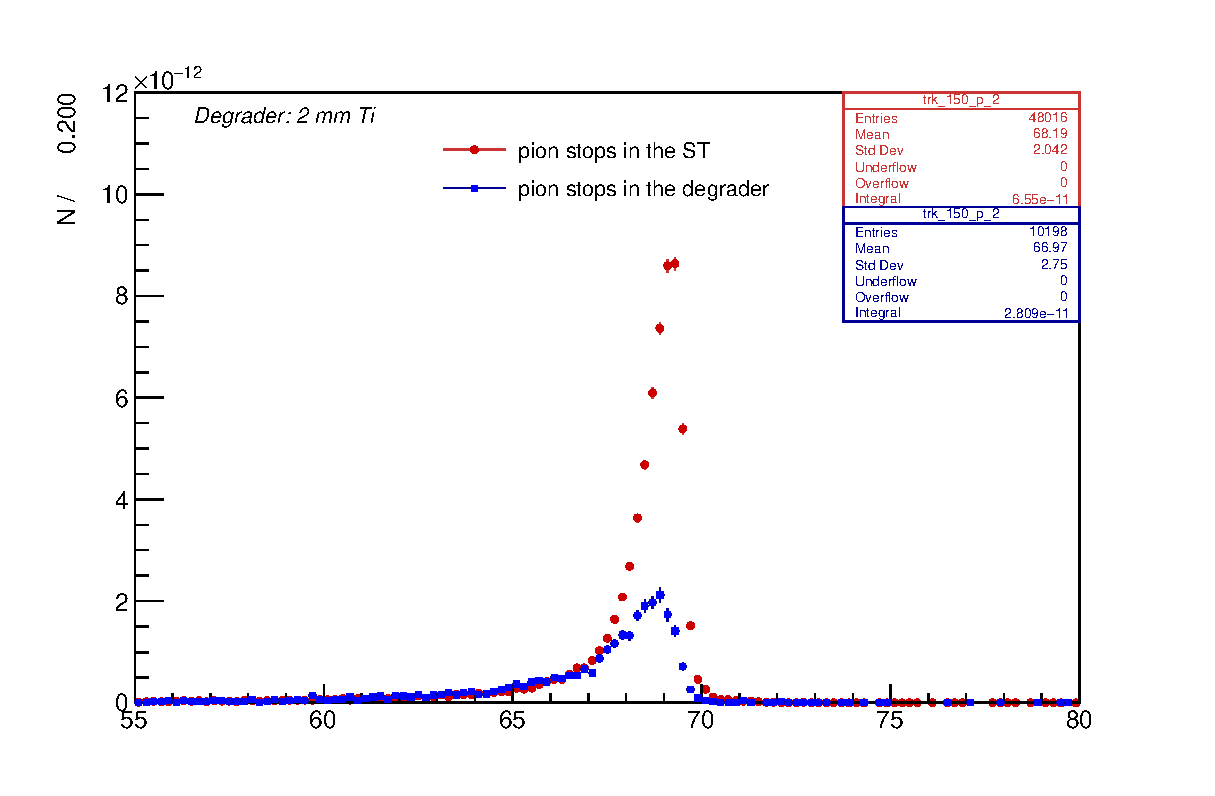
\includegraphics[width=0.55\linewidth]{pdf/figure_00251}
%   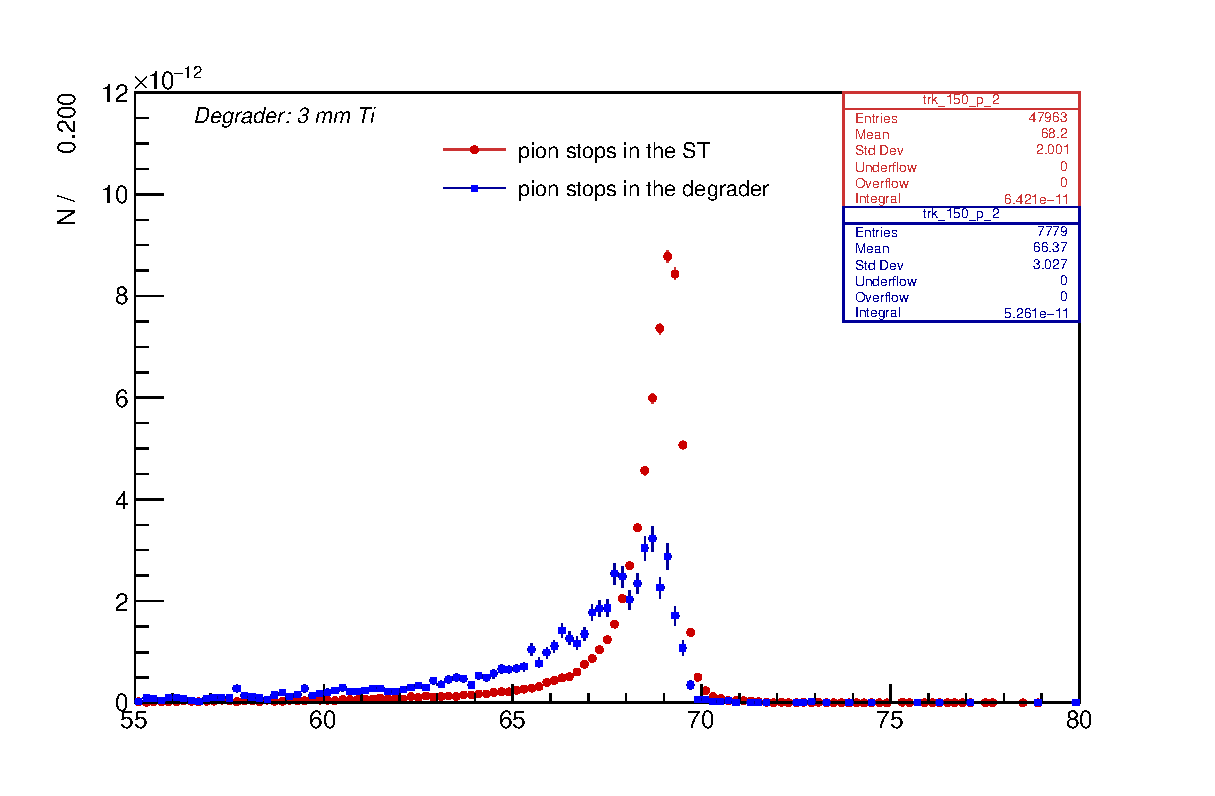
\includegraphics[width=0.55\linewidth]{pdf/figure_00351}
%   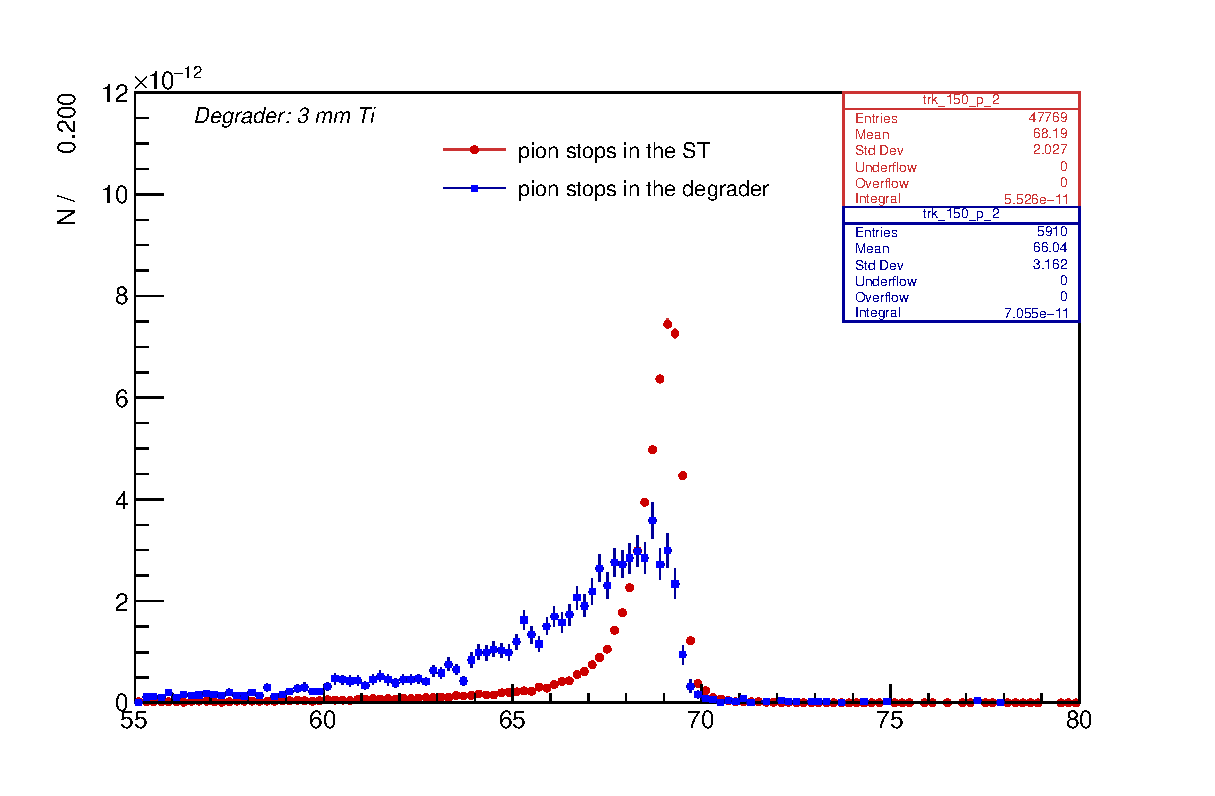
\includegraphics[width=0.55\linewidth]{pdf/figure_00451}
%   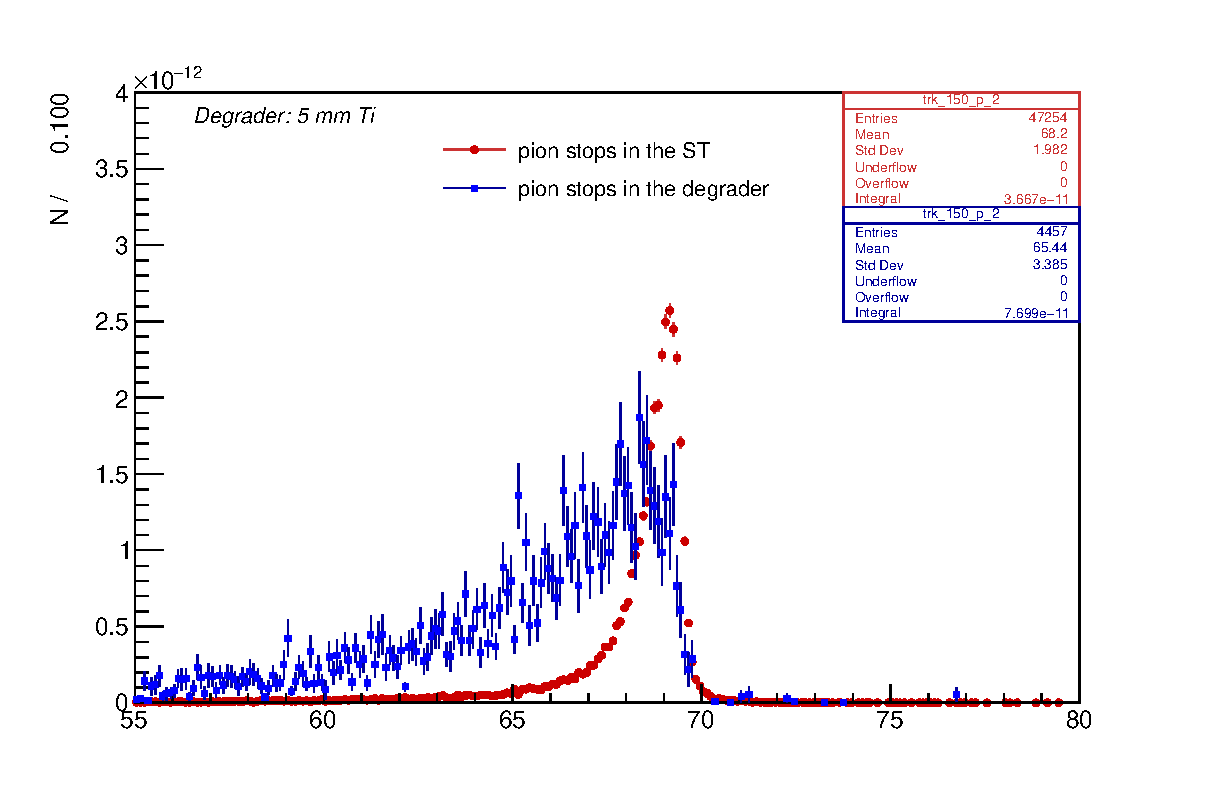
\includegraphics[width=0.55\linewidth]{pdf/figure_00551}
%   \caption{
%     % \label{fig:deg_vs_no_degrader_time}
%   }
% \end{figure}

\begin{figure}[H]
  % \centering
  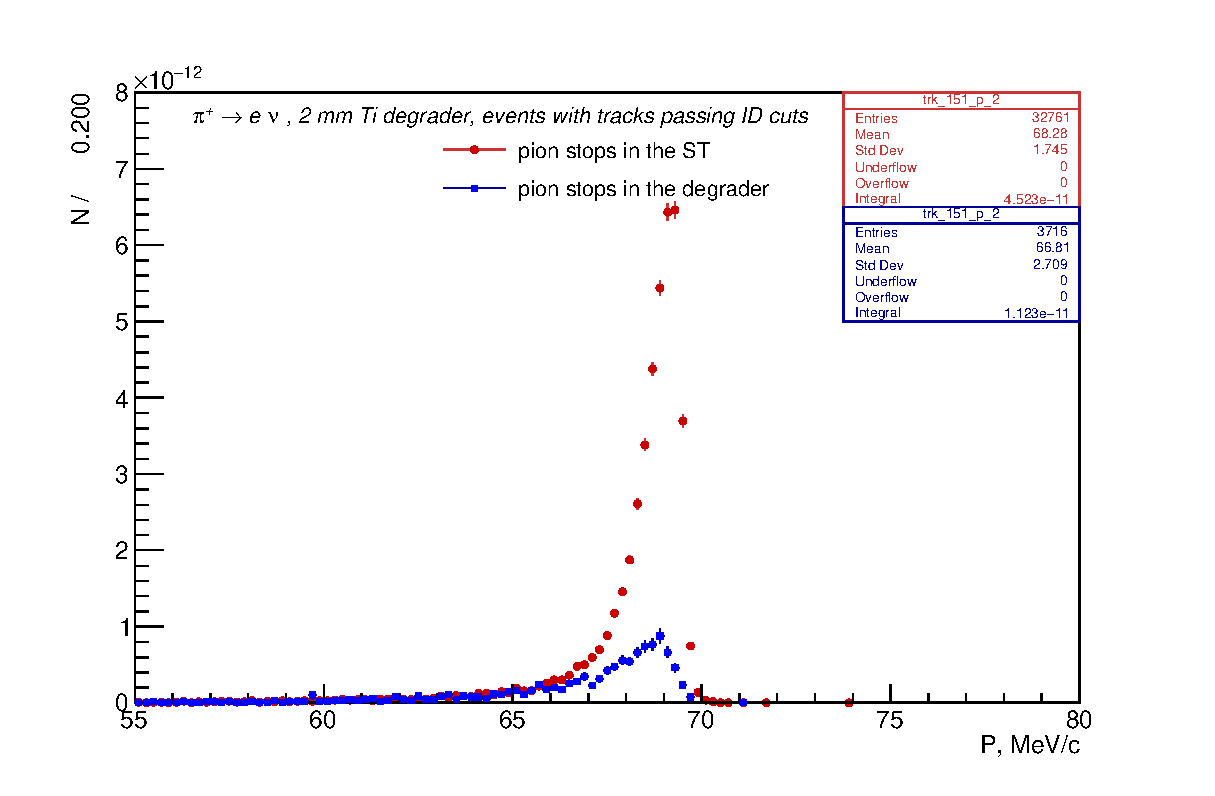
\includegraphics[width=0.55\linewidth]{pdf/figure_00261}
  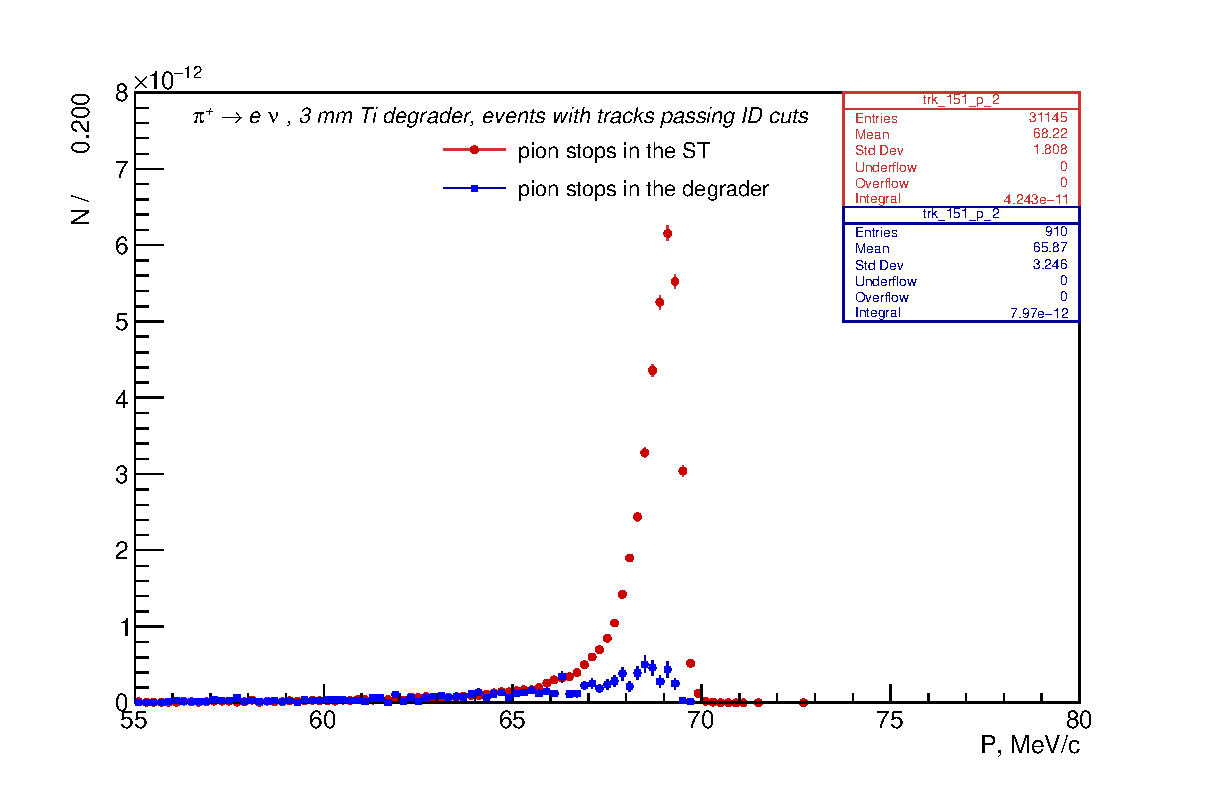
\includegraphics[width=0.55\linewidth]{pdf/figure_00361}
  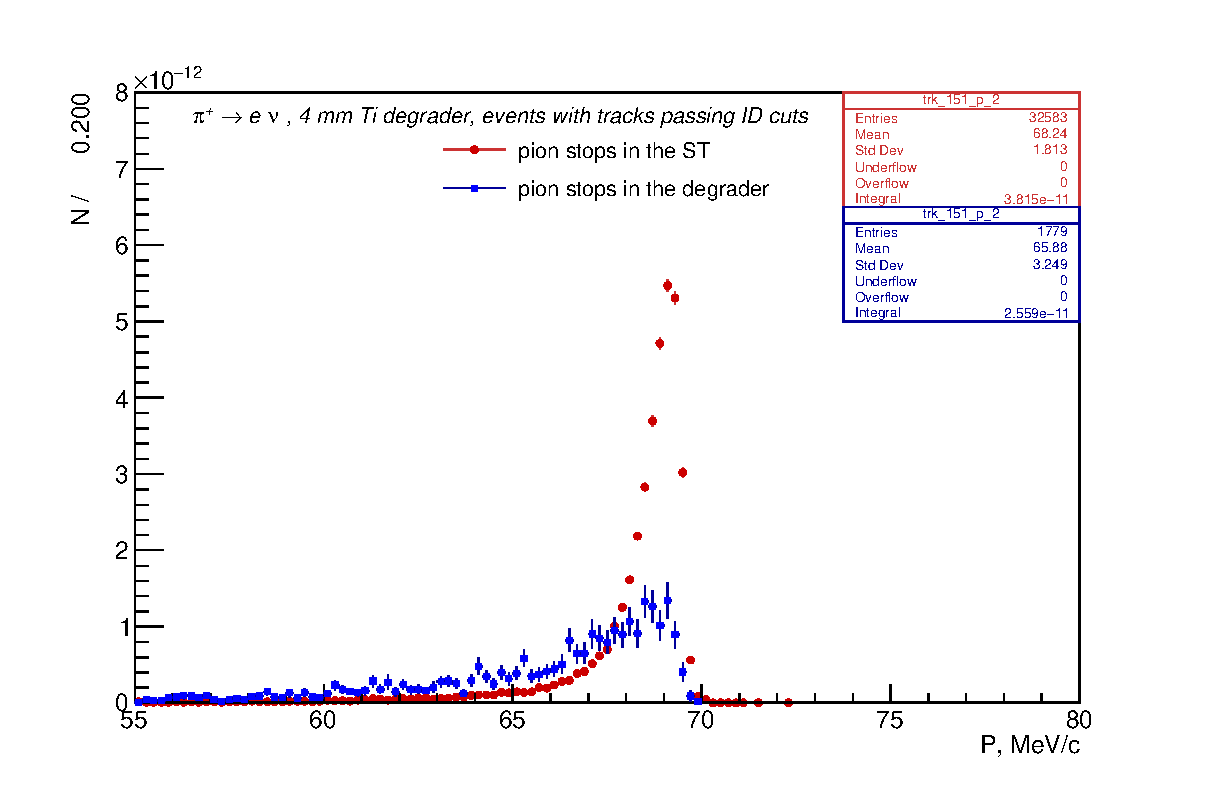
\includegraphics[width=0.55\linewidth]{pdf/figure_00461}
  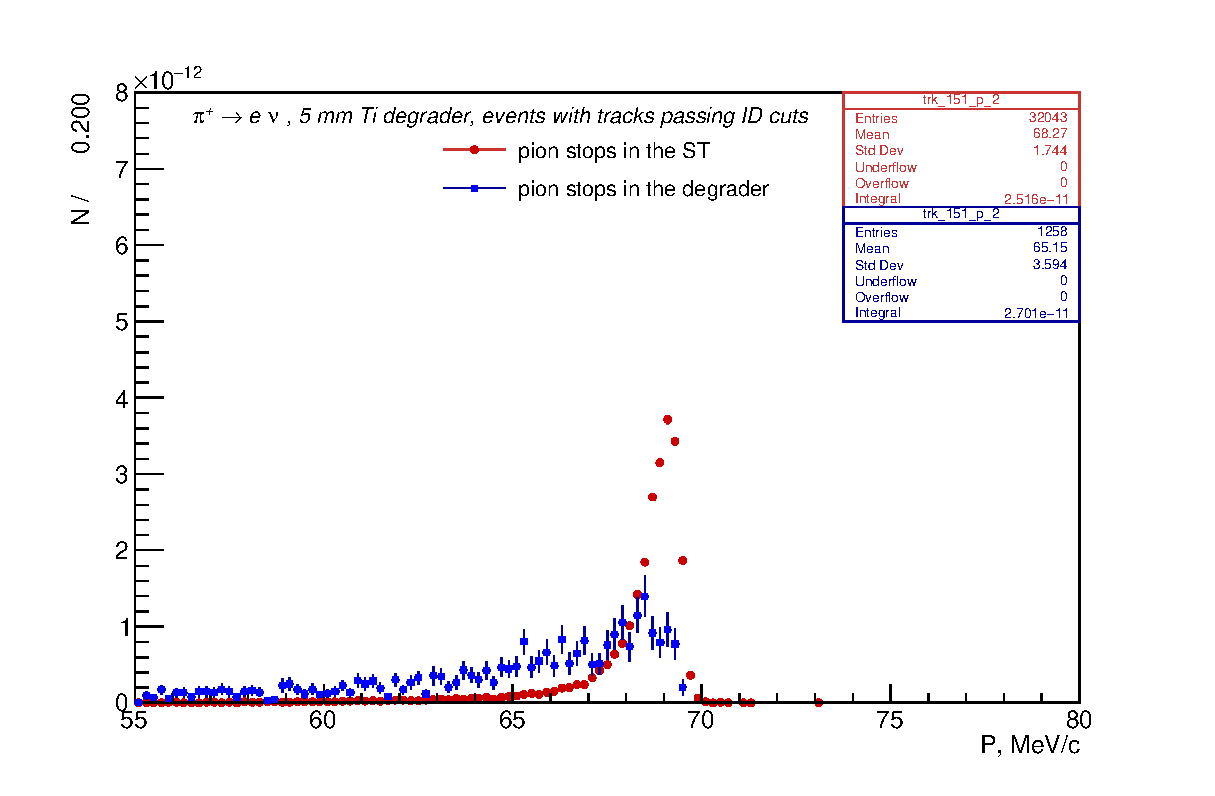
\includegraphics[width=0.55\linewidth]{pdf/figure_00561}
  \caption{
    \label{fig:stt_vs_deg_momentum_good_tracks}
    reconstructed e+ yield/POT for different degrader thicknesses, STT vs DEG
  }
\end{figure}

For the signal window $67.5 < P < 70$ MeV/c, the relative contribution of pion
decays in degrader is in the range of 10-15\%.

Timing distributions for tracks from \piplusenu\ decays in the ST and degrader and
passing the selection cuts are shown if Figure~\ref{figure:stt_vs_deg_t0_good_tracks}.
As, on average, slower pions stop in the degrader, the timing distributions 
of decays in the degrader fall a little bit slower.
Therefore, at large T0 the contribution of the degrader stops increases.


\begin{figure}[H]
  % \centering
  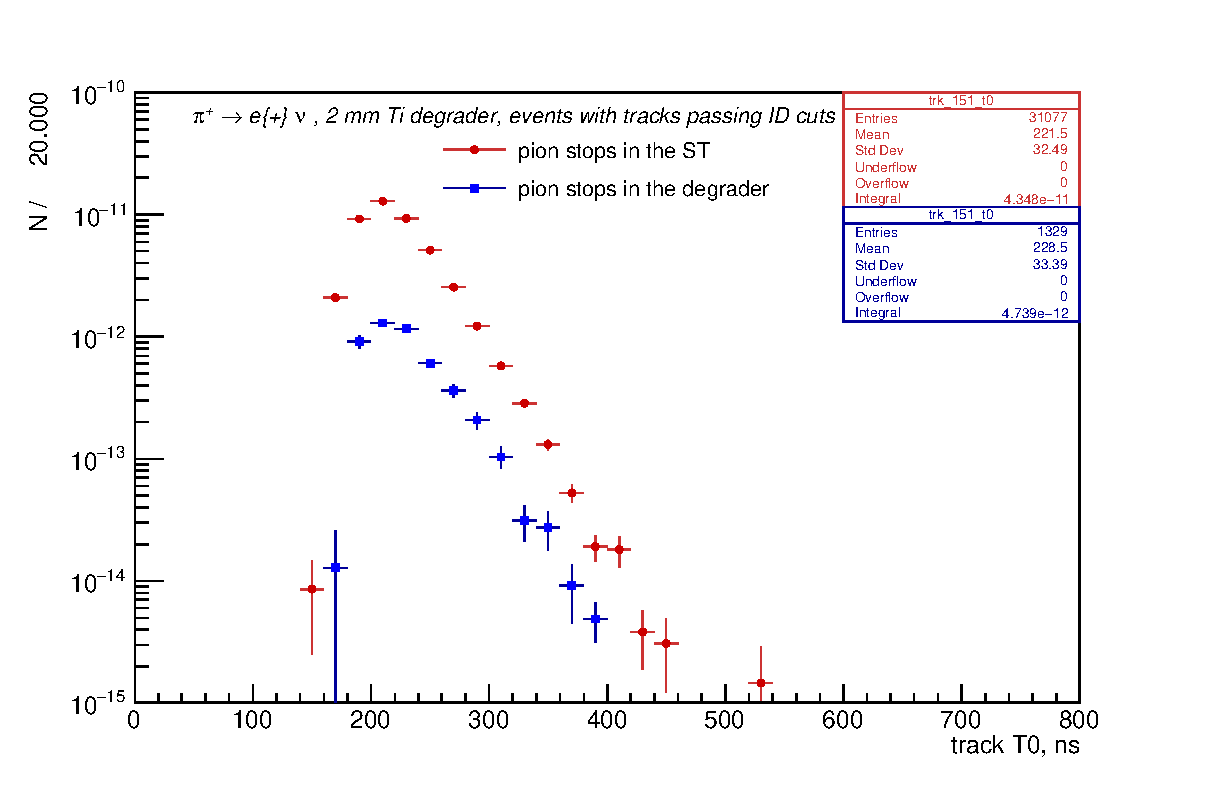
\includegraphics[width=0.55\linewidth]{pdf/figure_00262}
  \includegraphics[width=0.55\linewidth]{pdf/figure_00362}
  \includegraphics[width=0.55\linewidth]{pdf/figure_00462}
  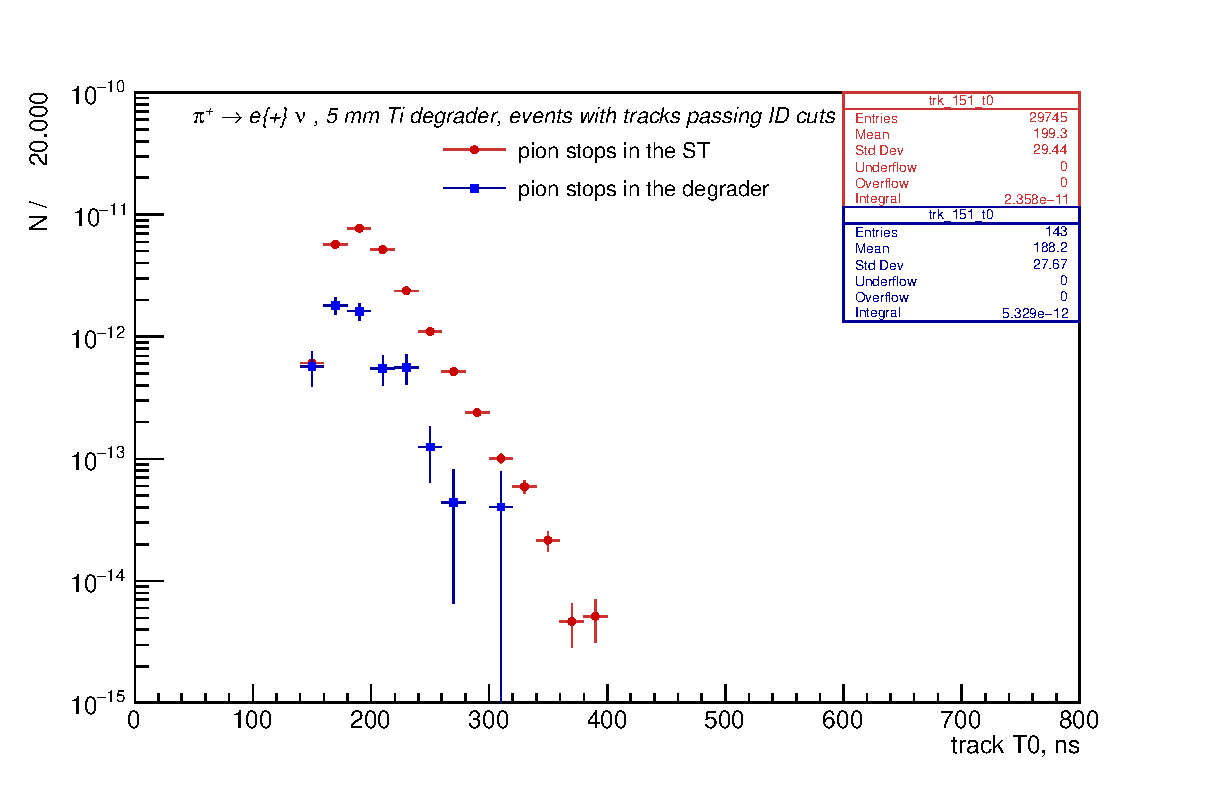
\includegraphics[width=0.55\linewidth]{pdf/figure_00562}
  \caption{
    \label{figure:stt_vs_deg_t0_good_tracks}
    reconstructed e+ yield/POT for different degrader thicknesses, STT vs DEG
  }
\end{figure}

%%%%%%%%%%%%%%%%%%%%%%%%%%%%%%%%%%%%%%%%%%%%%%%%%%%%%%%%%%%%%%%%%%%%%%%%%%%%%%
\subsection{Standard selection - results}

Figure~\ref{figure:no_deg_mom} shows momentum distributions of reconstructed
positron tracks from positive pion decays in the ST and muon decays in flight
for the detector configuration w/o the degrader. 
The tracks are required to pass the selection cuts and have the T0 > 300 ns. 
The \piplusenu\ signal is expected to be buried deep under the DIF background.

\begin{figure}[H]
  % \centering
  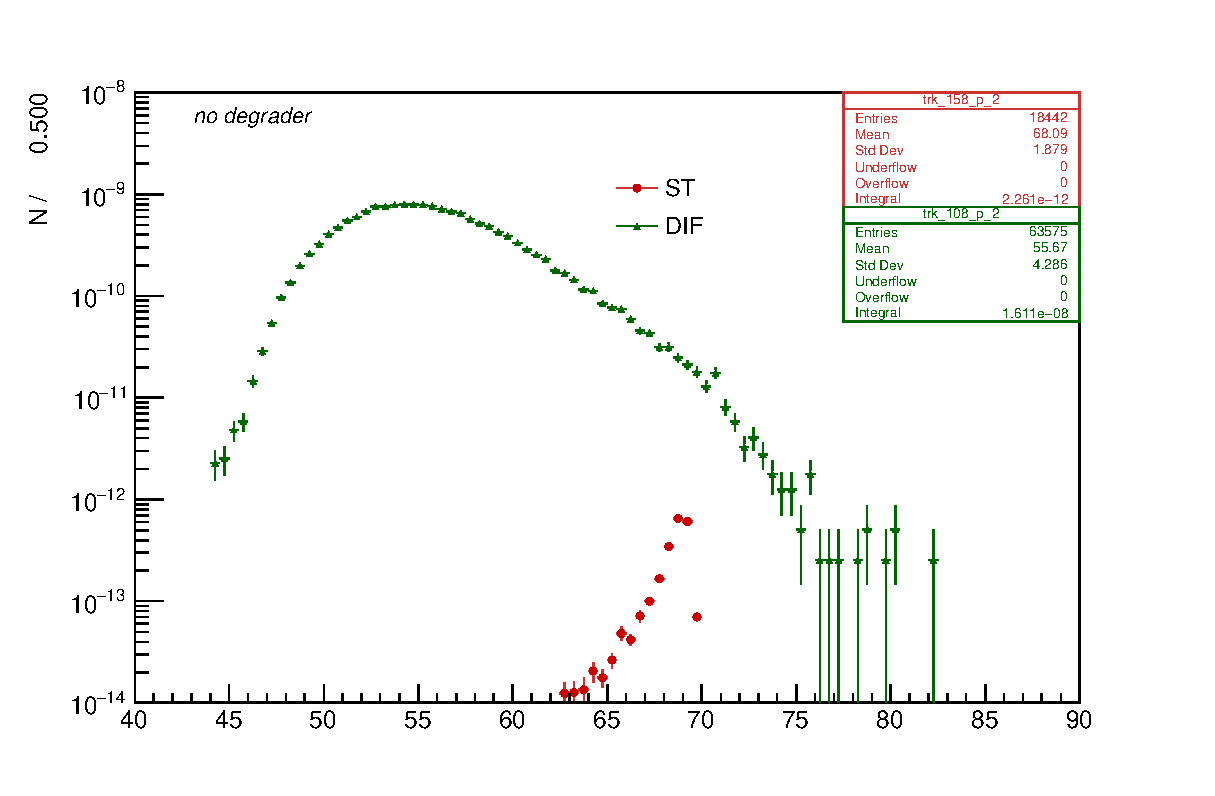
\includegraphics[width=0.90\linewidth]{pdf/figure_00031}
  \caption{
    \label{figure:no_deg_mom}
  }
\end{figure}

Distributions for different degrader thicknesses after T0>300 ns cut are shown
in Figure~\ref{figure:deg_mom}

\begin{figure}[H]
  % \centering
  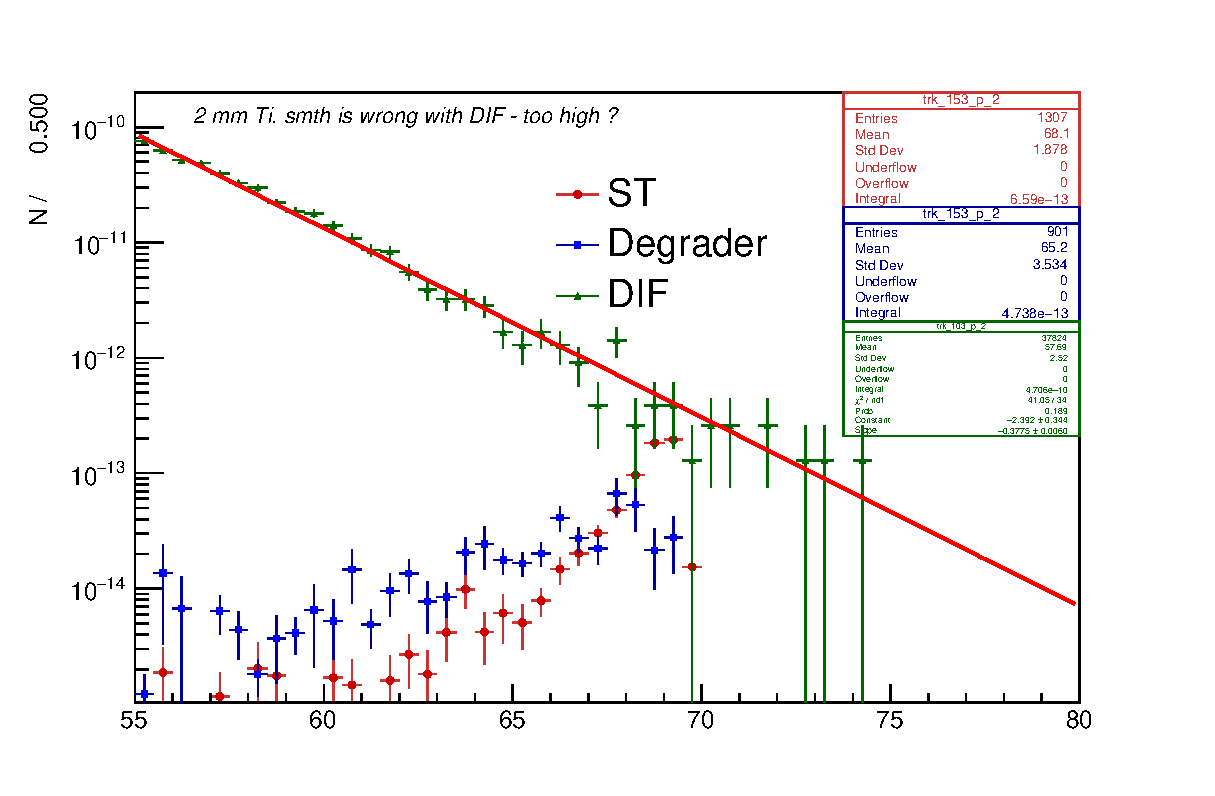
\includegraphics[width=0.55\linewidth]{pdf/figure_00231}
  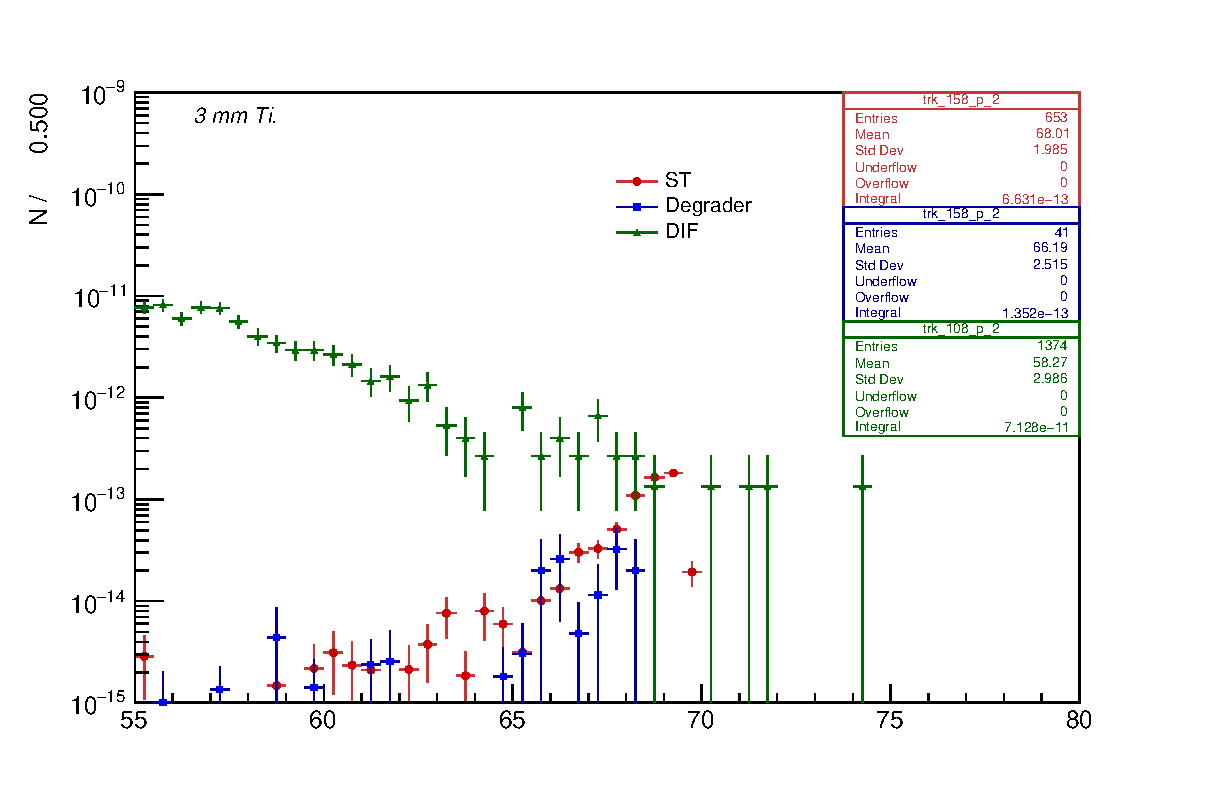
\includegraphics[width=0.55\linewidth]{pdf/figure_00331}
  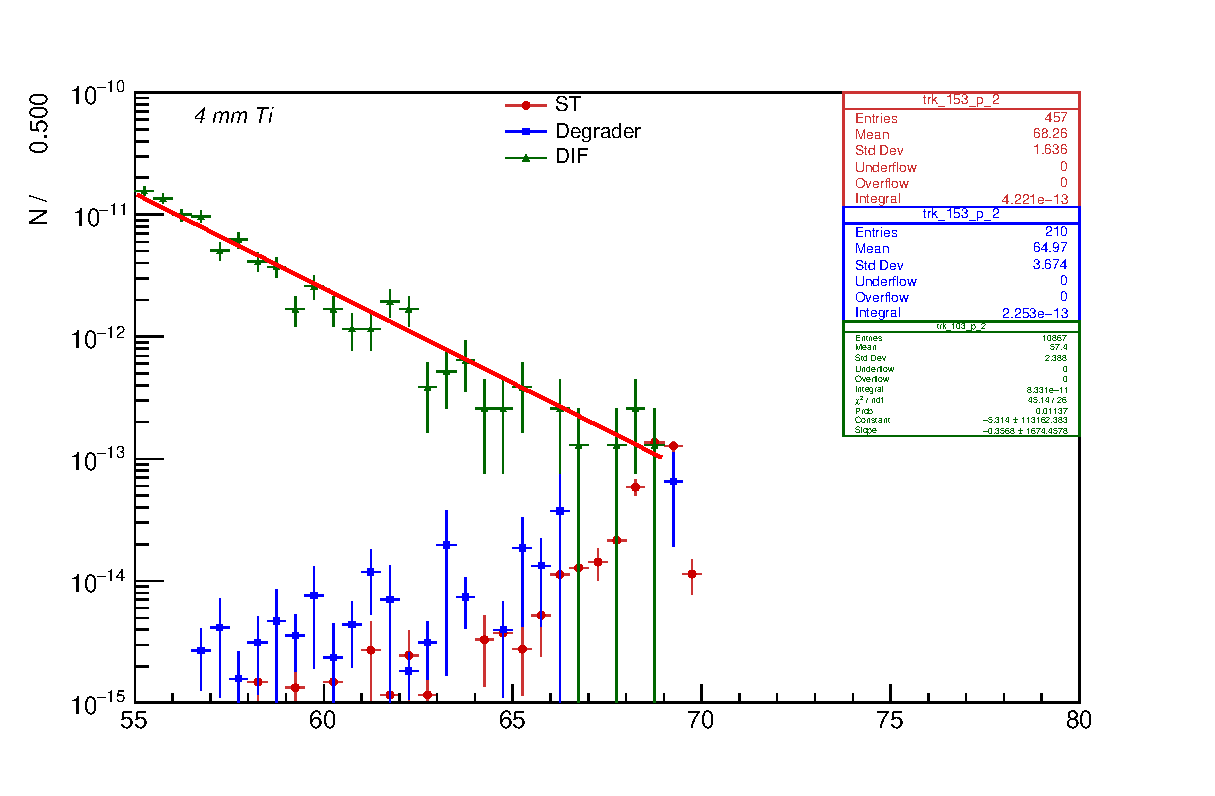
\includegraphics[width=0.55\linewidth]{pdf/figure_00431}
  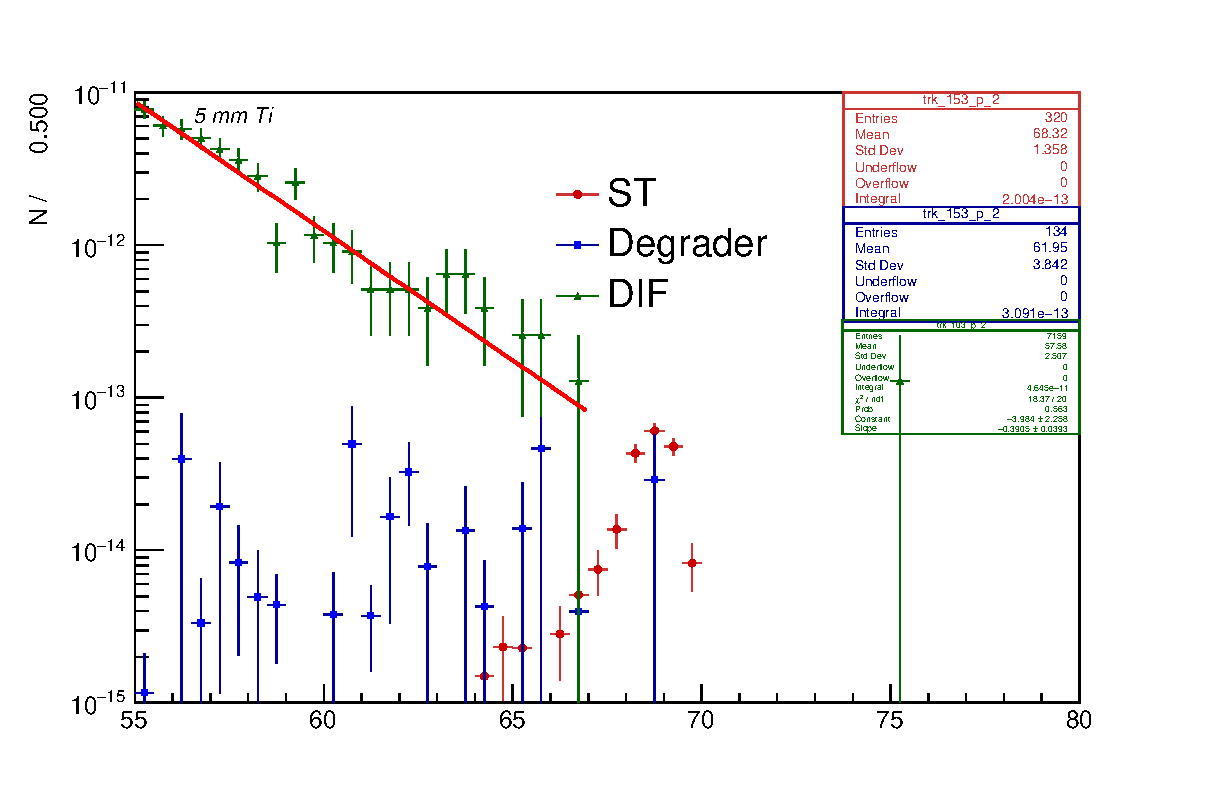
\includegraphics[width=0.55\linewidth]{pdf/figure_00531}
  \caption{
    \label{figure:deg_mom}
  }
\end{figure}

The signal vs background situation looks more promising, however thre is no clear indication
that the \piplusenu\ signal would be clearly seen on top of the DIF background.
The plots also do not indicate that increasing the degrader thickness from 2mm to 5mm 
improves  the signal to background ratio (S/B) in any significant way - the available
statistics is not sufficient for drawing such a conclusion.

For degrader thickness of 4mm, a visual scan of DIF events surviving
the selection cuts and having  hte reconstructed positron momentum above 65 MeV/c
has been performed.
%
The surviving events are dominated by correctly reconstructed events on the high-momentum tail
of the $\mu^+$ decays-in flight spectrum, and not by mis-reconstructed events.

%%% Local Variables:
%%% mode: latex
%%% TeX-master: "mu2e-xxxxx"
%%% End:


\appendix

%%%%%%%%%%%%%%%%%%%%%%%%%%%%%%%%%%%%%%%%%%%%%%%%%%%%%%%%%%%%%%%%%%%%%%%%%%%%%%
\section {Pion Yields}
\label{appendix_a}

\begin{tabularx}{1.0\textwidth} {|X|c|c|c|c|}  %
% \begin{tabular}{1.0\textwidth} {|l|l|}  %
  \hline
  Dataset             & Ti degrader thickness (mm)  & N(POT)     & N(ST stops) & N(DEG stops) \\
  \hline            
  bpip0b0             &  no degrader                & $2.5 10^8$ &             &               \\
  \hline
  bpip2b0             &              2              &            &             &               \\
  \hline
  bpip3b0             &                3            &            &             &                \\
  \hline
  bpip4b0             &          4                  &            &             &                \\
  \hline
  bpip5b0             &           5                 &            &             &                \\
  \hline
\end{tabularx}

% \makebox[\textwidth] {
{\tiny{
\begin{verbatim}
|-----------------+----------+--------+----------+--------+-----------------------+------------------+-----------|
| dataset         | degrader | N(POT) | N(stops) | N(sim) | SF=(Nstops/Nsim)/NPOT | BR(pi+ -> e+ nu) |  Total SF |
|-----------------+----------+--------+----------+--------+-----------------------+------------------+-----------|
| bpip0b0s21r0000 | none     |  2.5e8 |   312616 |    1e5 |             1.250e-08 |          1.23e-4 | 1.538e-12 |
| bpip2b0s21r0000 | 2 mm Ti  |  2.5e8 |    84785 |    1e5 |             3.391e-09 |          1.23e-4 | 4.171e-13 |
| bpip3b0s21r0000 | 3 mm Ti  |  2.5e8 |    50340 |    1e5 |             2.014e-09 |          1.23e-4 | 2.477e-13 |
| bpip4b0s21r0000 | 4 mm Ti  |  2.5e8 |    31681 |    1e5 |             1.267e-09 |          1.23e-4 | 1.558e-13 |
| bpip5b0s21r0000 | 5 mm Ti  |  2.5e8 |    17225 |    1e5 |             6.890e-10 |          1.23e-4 | 8.475e-14 |
|-----------------+----------+--------+----------+--------+-----------------------+------------------+-----------|
| bpip2b0s24r0000 | 2 mm Ti  |  2.5e8 |   448131 |    1e5 |             1.793e-08 |          1.23e-4 | 2.205e-12 |
| bpip3b0s24r0000 | 3 mm Ti  |  2.5e8 |   532767 |    1e5 |             2.131e-08 |          1.23e-4 | 2.621e-12 |
| bpip4b0s24r0000 | 4 mm Ti  |  2.5e8 |   583855 |    1e5 |             2.335e-08 |          1.23e-4 | 2.872e-12 |
| bpip5b0s24r0000 | 5 mm Ti  |  2.5e8 |   617324 |    1e5 |             2.469e-08 |          1.23e-4 | 3.037e-12 |
|-----------------+----------+--------+----------+--------+-----------------------+------------------+-----------|
#+TBLFM: $6=$4/$5/$3;%11.3e::$8=$6*$7;%11.3e::
\end{verbatim}
}
}

%%% Local Variables:
%%% mode: latex
%%% TeX-master: "mu2e-xxxxx"
%%% End:


%%%%%%%%%%%%%%%%%%%%%%%%%%%%%%%%%%%%%%%%%%%%%%%%%%%%%%%%%%%%%%%%%%%%%%%%%%%%%% 
\section {Summary}
%%%%%%%%%%%%%%%%%%%%%%%%%%%%%%%%%%%%%%%%%%%%%%%%%%%%%%%%%%%%%%%%%%%%%%%%%%%%%%
%
%%%%%%%%%%%%%%%%%%%%%%%%%%%%%%%%%%%%%%%%%%%%%%%%%%%%%%%%%%%%%%%%%%%%%%%%%%%%%%
\newpage
\bibliographystyle{unsrtnat}
\bibliography{clfv,mu2e_internal_notes,statistics}
\end{document}
